\section{Driver Amplifier}

First, the Driver Amplifier was built. The associated schematic can be
seen in Figure~\ref{DriverAmp}.

\begin{figure}[h!]
  \centering
  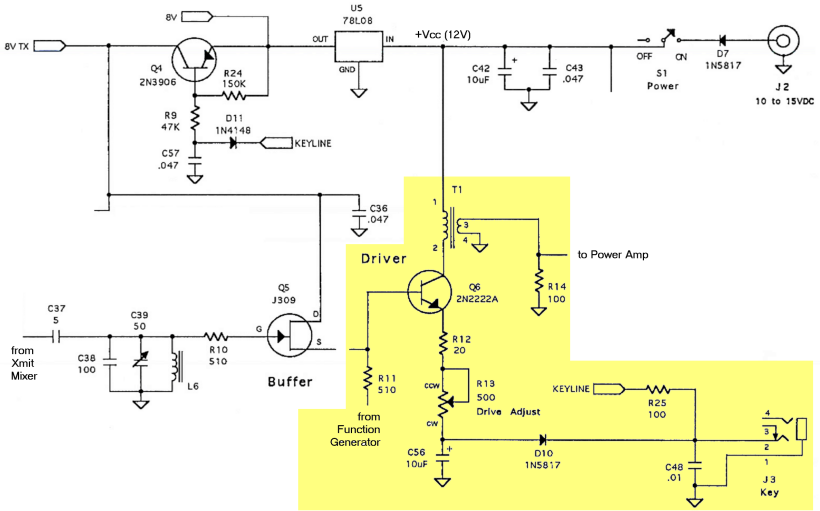
\includegraphics[scale=0.6]{./img/DriverAmp.png}
  \label{DriverAmp}
  \caption{Circuit Schematic for the Driver Amplifier}
\end{figure}

\subsection{Measured Output Voltage: \bm{$V_{pp}$}}
With the function generator set to 7.04MHz, and with an offset of 
%Remember to edit this if any changes are made!
$0.5V$. The output voltage across $R_{14}$ was measured to be $\boxed{ V}$.

\subsection{Calculated Output Power: \bm{$P$}}
  $P$ is calculated using the following:

  \begin{align*}
    P &= \frac{V_{pp}^2}{8( 50\Omega||R_{14})}\approx
    \frac{V_{pp}^2}{267\Omega}\\
  \therefore  P &= \boxed{ mA}
  \end{align*}
  %Since $V_{cc}$ is given as $12V$, $R_{14} = 100 \Omega$ and transformer $T_1$ has a turns ratio $n =
  %\frac{14}{4} = 3.5$:
  %\begin{align*}
  %  P &= \frac{12^2}{(3.5^2 \cdot 100}) = \boxed{117.5 mW}
  %\end{align*}
\subsection{Calculated Supply Power: \bm{$P_{0}$}}
\subsubsection{\bm{$V_{R_{12}}$}} 
  The DC voltage across $R_{12}$, $V_{R_{12}}$ was recorded to be $\boxed{ V}$.
  \subsubsection{\bm{$i_E$}}
  The emitter current, $i_E$, was found by:
  \begin{align*}
    i_E &= \frac{V_{R_{12}}}{R_{12}}=\boxed{ mA}
  \end{align*}
  \subsubsection{Supply Power: \bm{$P_0$}}
    $V_{cc}$ was measured at the $1\Omega$ resistor across $S_1$, and found to
    be $\boxed{ V}$ Therefore, the DC supply power $P_0 = (V_{cc}\cdot i_E)=\boxed{ mW}$

\subsection{System Efficiency: \bm{$\eta$}}
  The efficiency $\eta$ was calculated to be:
  \begin{align*}
    \eta &= \frac{P}{P_0} = \boxed{ } = \boxed{ \%} 
  \end{align*}

\subsection{Amplifier Gain: \bm{$G$}}
  The gain $G$ was found to be:
  \begin{align*}
    G &= 10log\bigg(\frac{P}{P_{+}}\bigg) \text{dB}\\
    P_{+} &=  \frac{V_{+pp}^2}{8R_s}\\
    V_{+pp} &\equiv \text{Function Generator Amplitude}\\
    R_s &= 50\Omega\\
    \therefore G &= \boxed{ \text{dB}}
  \end{align*}
\subsubsection{}
When $R_{13}$ is fully clockwise (max), the voltage gain was found to be:
$G_{v\,(Max)} = \bigg(\dfrac{v}{v_i}\bigg) = \boxed{}$.
\subsubsection{}
When $R_{13}$ is fully counter-clockwise (min), the voltage gain was found to be:
$G_{v\, (Min)} = \bigg(\dfrac{v}{v_i}\bigg) = \boxed{}$.

\subsection{Miller Capacitance, \bm{$C_M$}}

Using $G_{v\,(Max)}$, the Miller Capacitance, $C_M$ was found using:

\begin{align*}
 C_M &=
\end{align*}

(\emph{Note:} At the end of this step, the other end of $R_{11}$ was soldered).
